\documentclass[a4paper,12pt]{article}

\usepackage{rotating}
\usepackage[top=1in, bottom=1in, left=0.75in, right=0.75in]{geometry}
\usepackage{graphicx}
\usepackage[numbers,square,sort&compress]{natbib}
\usepackage{setspace}
\usepackage[cdot,mediumqspace,]{SIunits}
\usepackage{caption}
\usepackage{subcaption}
\usepackage{mathtools}
\usepackage{authblk}
\usepackage{float}
\renewcommand{\thesubsection}{\thesection.\alph{subsection}}
\providecommand{\e}[1]{\ensuremath{\times 10^{#1}}}

\begin{document}
\onehalfspacing
\title{PHY 407 Lab 11}
\author{Natalie Price-Jones, 999091021}
\date{28 November 2014}
\affil{\small{natalie.price.jones@mail.utoronto.ca}}
\maketitle

\section{Question 1}

\begin{figure}[H]
\centering
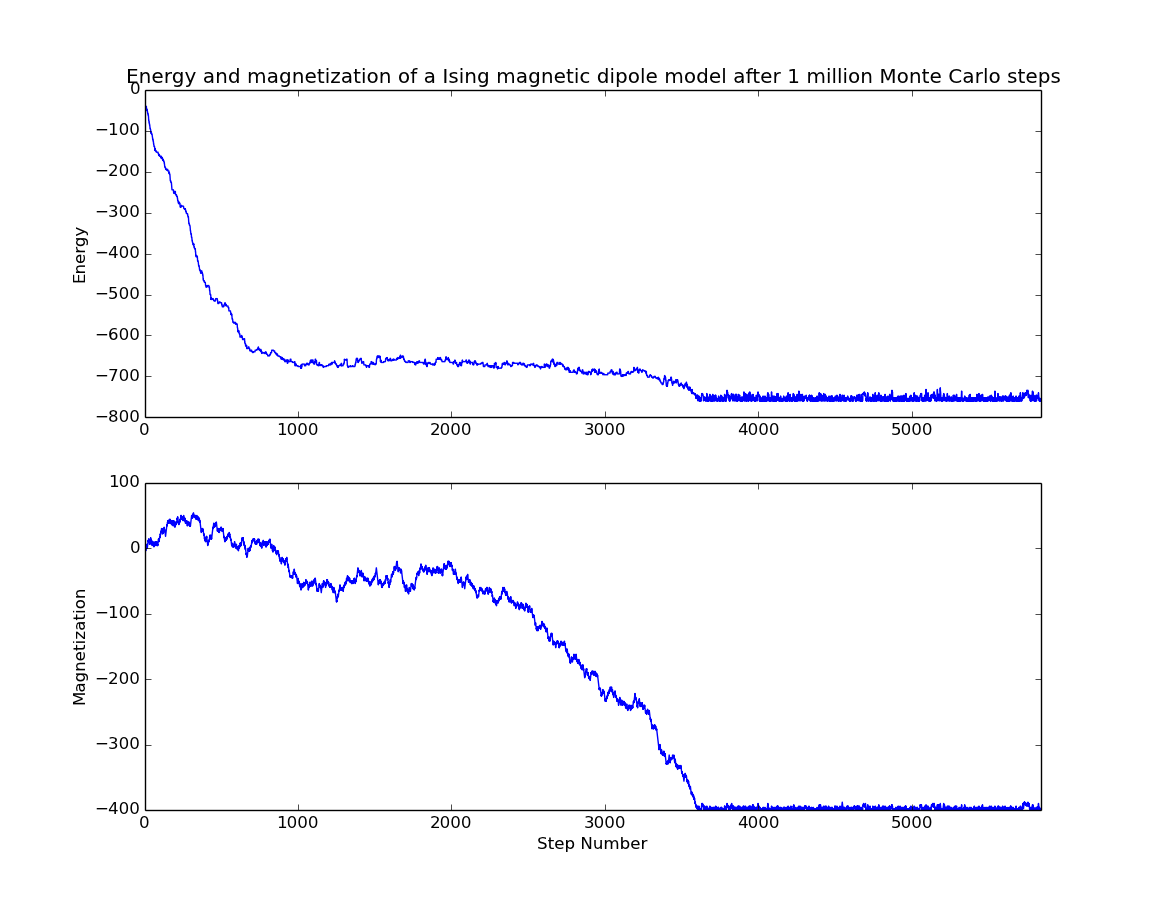
\includegraphics[width = \linewidth]{lab11q1.png}
\caption{}
\label{fig:q1}
\end{figure}


\section{Question 2}

Response to part d): Each time program is run, it develops either a positive or negative magnetization, but there is no way to predict from the outset, which this will be, unless the starting distribution is remarkably non uniform (which can happen, even when randomly assigning spin). Since the process of flipping the spin of a random dipole is itself inherently random, the dominant spin is unpredictable from the outset. There were even instances where it seemed that one spin was dominant, but it would eventually lose to the other. So for an appropriate temperature, the final result is always that all dipoles have the same spin, but the direction of that spin (and hence the sign of the magnetization), is generally a 50:50 split between the two options.

\begin{figure}[H]
\centering
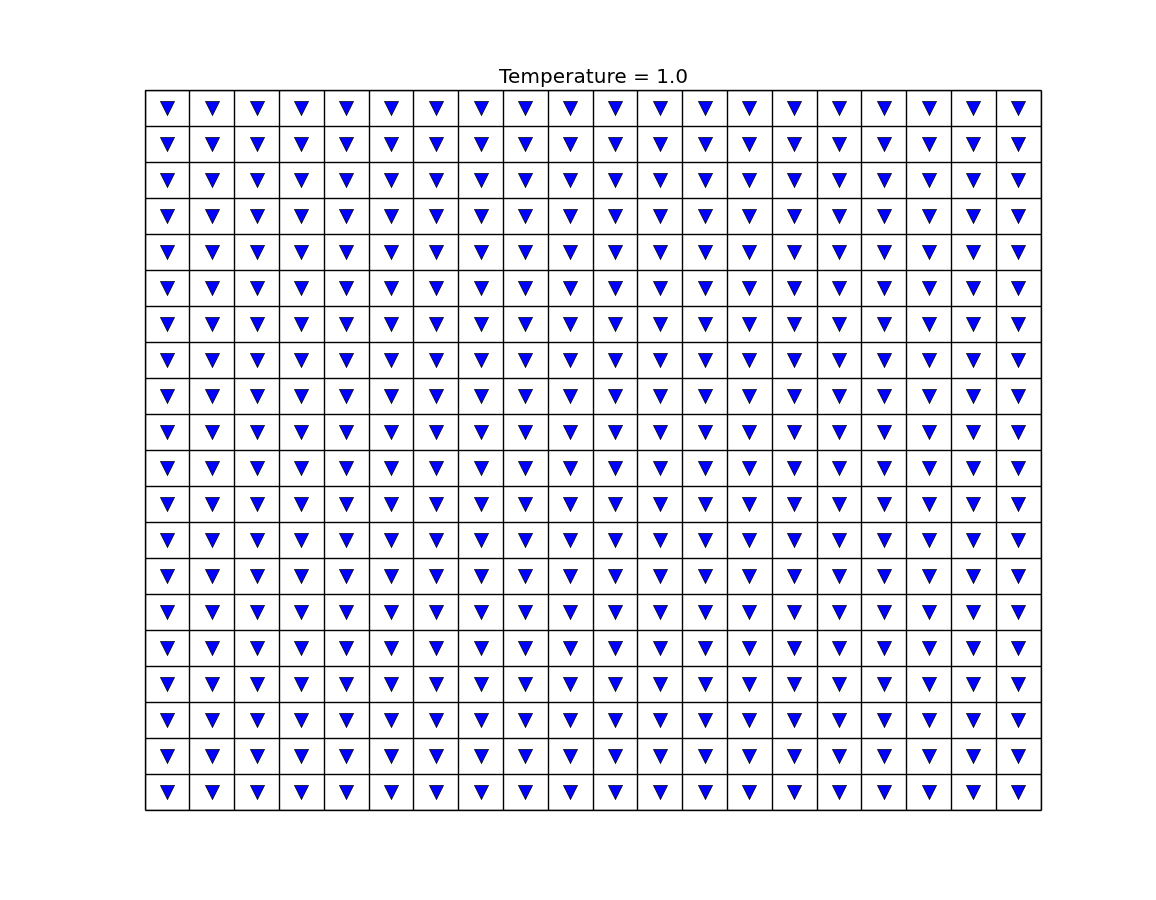
\includegraphics[width = \linewidth]{lab11q2.png}
\caption{}
\label{fig:q2}
\end{figure}

\begin{figure}[H]
\centering
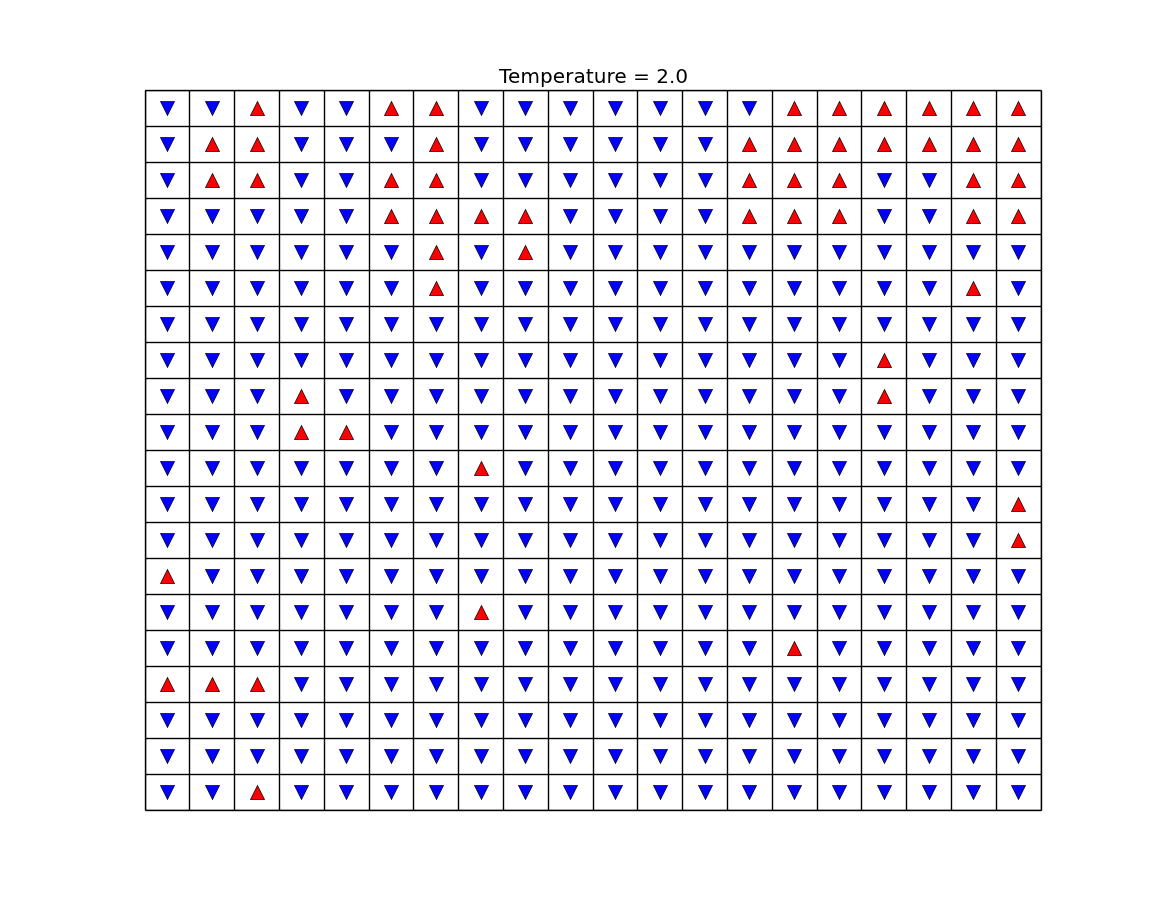
\includegraphics[width = \linewidth]{lab11q2_2.png}
\caption{}
\label{fig:q2_2}
\end{figure}

\begin{figure}[H]
\centering
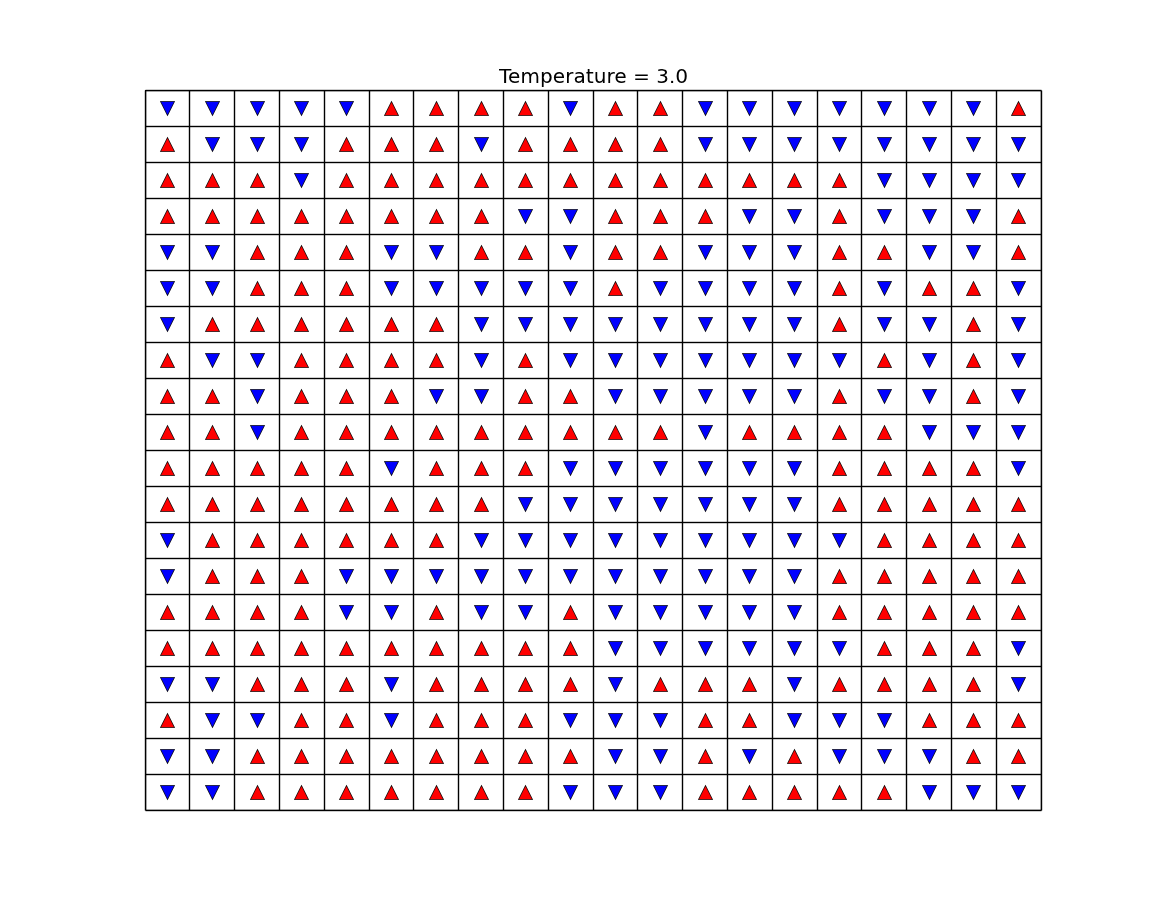
\includegraphics[width = \linewidth]{lab11q2_3.png}
\caption{}
\label{fig:q2_3}
\end{figure}


\section{Question 3}

\begin{figure}[H]
\centering
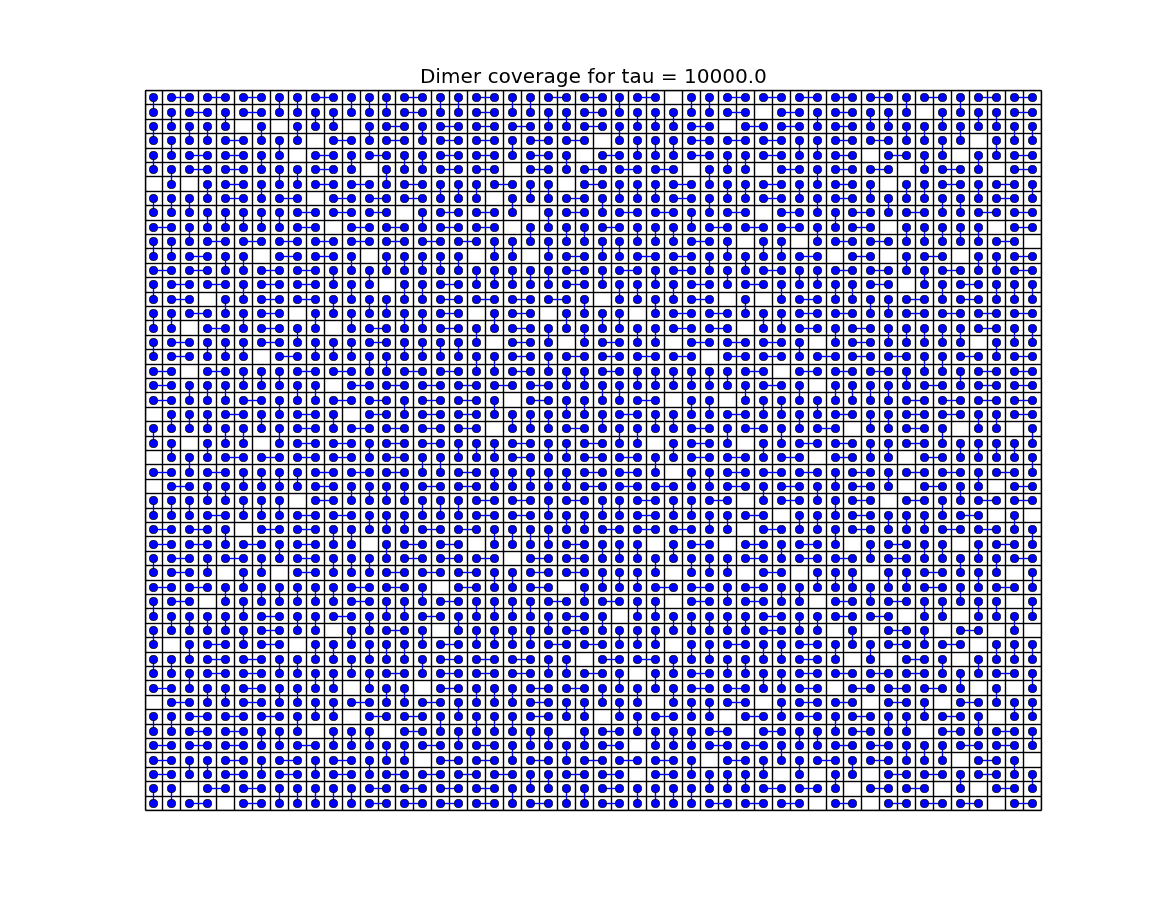
\includegraphics[width = \linewidth]{lab11q3_1e4.png}
\caption{}
\label{fig:q3_4}
\end{figure}

\begin{figure}[H]
\centering
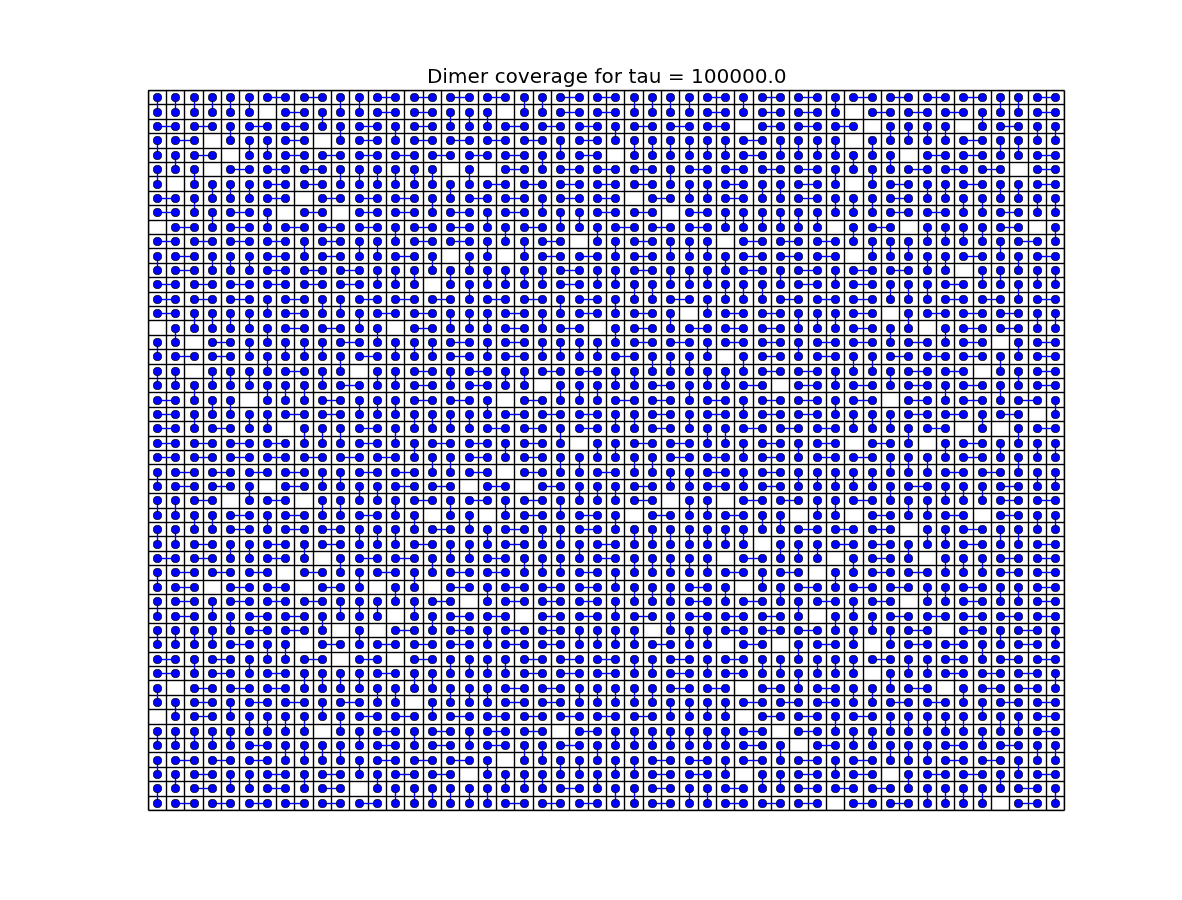
\includegraphics[width = \linewidth]{lab11q3_1e5.png}
\caption{}
\label{fig:q3_5}
\end{figure}

\begin{figure}[H]
\centering
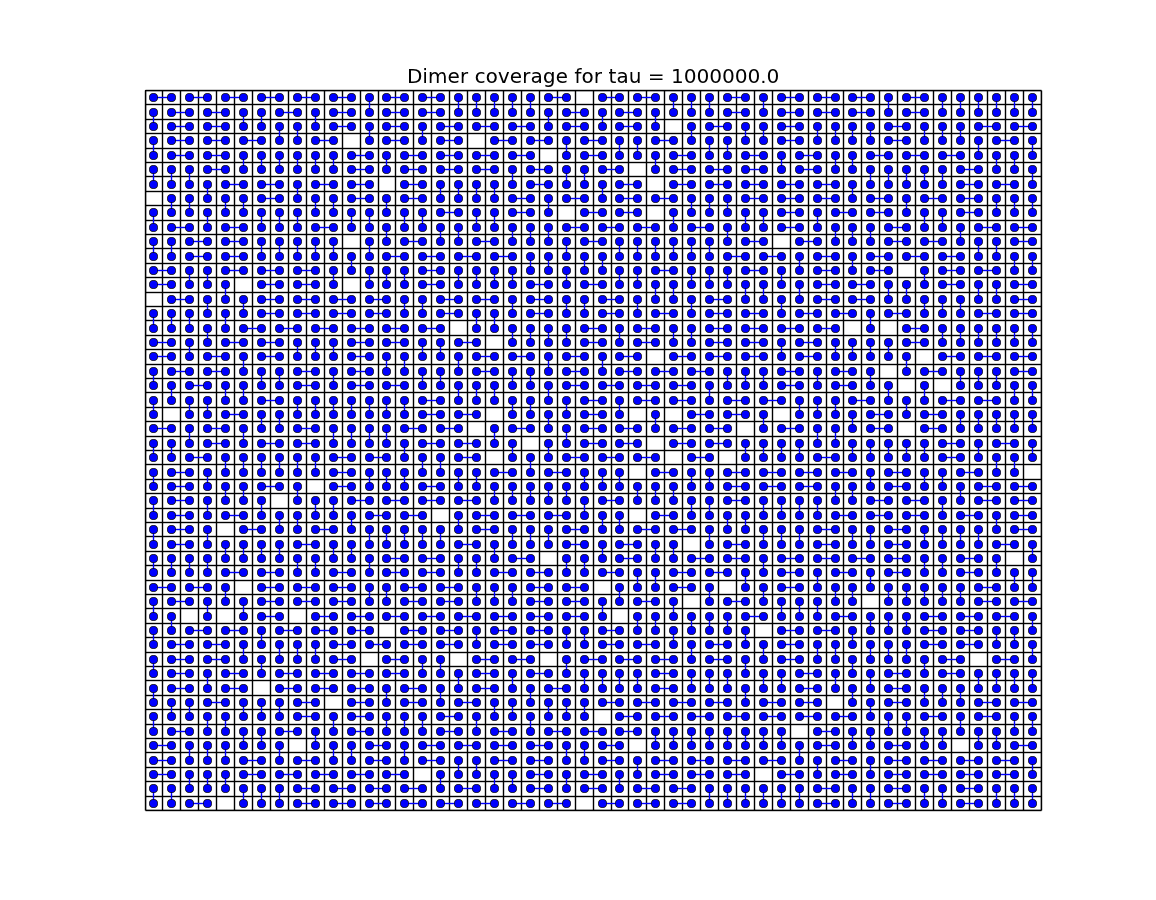
\includegraphics[width = \linewidth]{lab11q3_1e6.png}
\caption{}
\label{fig:q3_6}
\end{figure}



\end{document}